\documentclass{article}
\usepackage{marginnote}
\usepackage[margin=1.5in,heightrounded,marginparsep=.1in,marginparwidth=1.2in]{geometry}
\usepackage[dvipsnames]{xcolor}
% fonts:
\usepackage{fontspec}
\defaultfontfeatures{Ligatures=TeX,Numbers={OldStyle,Proportional}}
\setmainfont{XCharter}
\setsansfont{Alegreya Sans}
\newfontfamily\charis{CharisSIL-R.ttf}[
    BoldFont = CharisSIL-B.ttf,
    ItalicFont = CharisSIL-I.ttf,
    BoldItalicFont = CharisSIL-BI.ttf]
\usepackage[colorlinks]{hyperref}
\hypersetup{allcolors=Blue}
\usepackage{gb4e}
\usepackage{cgloss}
\noautomath
\let\eachwordone=\charis
%\usepackage{leipzig}
%\makeglossaries
\usepackage{amssymb}
\usepackage{fancyhdr}
\usepackage{authblk}
\setlength{\affilsep}{.2cm}
\usepackage{marvosym}
\usepackage[round]{natbib}
%\pagestyle{fancy}
\usepackage{graphicx}
\lhead{Towards a typology of quantification\\in Australian languages }\chead{}\rhead{ALW 2018}
\newcommand{\ofy}{/85} %@ the n of languages in the survey
\newcommand{\pn}{Pama-Nyungan}

\title{Towards a typology of quantification in\\ Australian languages\thanks{We thank Ed Keenan and Pam Munro for their feedback on this project. We also thank our UCLA research assistants, Nick Curleo and Ryan Smick, for their help collecting data!}}
\author{Margit Bowler\authorcr UCLA \and \vspace{-.5cm}Vanya Kapitonov\thanks{\Letter:~\href{mailto:moving.alpha@gmail.com}{moving.alpha@gmail.com}}\authorcr University of Melbourne}
% \author{Margit Bowler}
% \affil {UCLA}
% \author {Vanya Kapitonov\thanks{\Letter:~\href{mailto:moving.alpha@gmail.com}{moving.alpha@gmail.com}}}
% \affil {University of Melbourne \&\ CoEDL}
\date{Australian Languages Workshop\\4 March 2018}

\begin{document}

\maketitle

% Vanya, please feel free to change anything you think needs changing!

\section[Introduction]{Introduction}
\begin{itemize}
    \item In this talk, we give the preliminary results of our typological survey of quantifier terms in Australian languages.
    \item Australian languages are  frequently described as having ``simple'' or ``impoverished'' quantifier systems.% grammars and  extremely impoverished counting systems (`one,' `two,' `many').
    \item We show that Australian languages have a variety of quantificational expressions, contrary to this stereotype.
    \item Of particular interest is the variety of morphosyntactic strategies that Australian languages use for expressing quantificational concepts.
\end{itemize}

\subsection{Scope of our survey}

\begin{itemize}
    \item Our typology is based on data from 96 published grammars or grammatical sketches on 85  Australian languages.
    
    % 96 = # of sources that have data (everything but "no")
    % this includes more than one source per language; the actual # of languages in our sample is smaller
    
    % 90 = actual # of languages surveyed so far
    \item We aim to have a sample that is genetically and areally balanced.
    \begin{itemize}
           \item Our survey currently includes languages from all Australian states/territories except Tasmania and the Australian Capital Territory (6/8).
           %\footnote{The Australian Capital Territory is very small (think Washington DC) and we were unable to locate relevant data on the languages that are spoken there. Linguists generally do not have very much information on Tasmanian languages. The last speaker of a Tasmanian language passed away in 1905.}
             \item The {\bf Pama-Nyungan} family contains 90\% of the languages in Australia.
        
        \begin{itemize}
            \item There are $\sim$25-30 accepted subgroups in Pama-Nyungan (\citealt{bowernatkinson12,ogradyvoegelin66}). 
        \item Our study includes 50 Pama-Nyungan languages from 23 subgroups.
        \end{itemize}
        \item {\bf Non-Pama-Nyungan} families contain the remaining 10\% of languages in Australia; non-Pama-Nyungan languages are spoken only in northern Australia (NT and WA).
        \begin{itemize}
         \item There are $\sim$15-20 accepted families in non-Pama-Nyungan (\citealt[xv]{kn14}).
        \item Our study includes 31 non-Pama-Nyungan languages from 16 families.
        % What is our extra subgroup???
        \end{itemize}
 %   \vspace{-3mm}
    
\begin{figure}
    \centering
    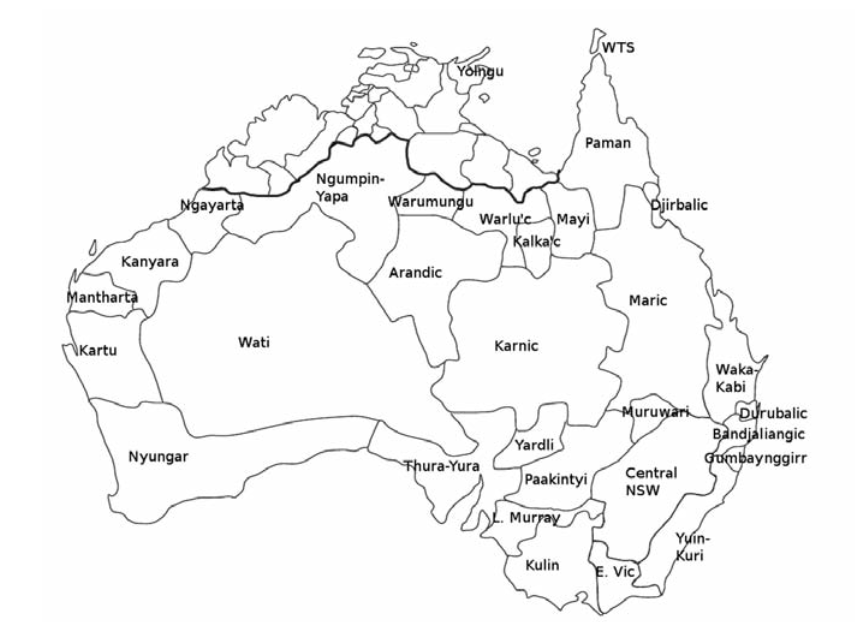
\includegraphics[scale=0.38]{pamanyunganmap1.png}
    \caption{Map of major current subgroups of Pama-Nyungan (\citealt[820]{bowernatkinson12})}
\end{figure}

   \begin{itemize} 
        \item We also include 8 language isolates (sometimes classified as isolates within either Pama-Nyungan or non-Pama-Nyungan, e.g.\ Muruwari, Wardaman) and 2 creoles.
    \end{itemize}
\end{itemize}
    \item When we report that a language ``has'' a quantifier, we mean that the source(s) that we consulted on the language describe this quantifier.
    \item We restrain from making strong claims about languages lacking certain quantificational expressions, since there may be gaps in the collected data.
    \item We instead present proportions. 
    
    \begin{itemize}
        \item For each expression we discuss, we show {\bf how many languages in our sample have it / the total number of languages for which we have quantifier data.}
        \item We surveyed a total of 109 sources; of these, only 96 had quantifier data.
    \end{itemize}
    
%        \item We focused primarily on sources published after 1980 to maximize the likelihood that the sources we consulted would include information on quantifiers.
        \item We generally present data as it is given in the source: We standardize some interlinear glosses, and generally use the author's chosen orthography.
    \end{itemize}
    
    \subsection{How we define quantifiers}
\begin{itemize}
    \item For the purpose of this study, we do not assume a theoretical definition of quantifiers (i.e., \citealt{heimkratzer98}).
    \item {\bf We define quantifiers as lexical items that refer to quantities, typically of individuals.}  This includes:
    
    % It is really hard to give a non-theoretical definition of quantifiers!!!! Please change this as you see fit! I don't like what I wrote.

    
\begin{itemize}
        \item Terms referring to vague quantities ({\it many, few, several, ...})
        \item Terms referring to properties of sets ({\it all, some, no,} ...)
        \item Terms referring to cardinalities ({\it one, two, three}, ...)
        \item Wh-words referring to quantities  ({\it how many, how much})
        \item Indefinite pronouns ({\it someone, something, somewhere, ...})
        \item Terms referring to ``quantities'' of times ({\it always, often, sometimes...})
\end{itemize}
    \item Our study does {\bf not} include:
\begin{itemize}
    \item Number marking in agreement systems, e.g.\ singular, dual, or paucal agreement
    \item Non-pronominal (in)definiteness
    \item Expressions that have been theoretically argued to include quantifiers in their semantic denotations, e.g.\ modals (\citealt{heimkratzer98})
\end{itemize}
\end{itemize}


\section{Morphosyntactic findings}
\label{sec:mpsfind}

\subsection{Lexical categories of quantifier terms}

\begin{itemize}
    \item The vast majority of languages in our survey encode quantifier terms as nouns.\footnote{Australian languages are often described as lacking adjectives, which pattern like nouns in e.g.\ hosting case marking and triggering agreement marking. Verbs and nouns tend to be the two major lexical categories.}
    \item Like other nouns, they can host case marking and trigger agreement marking.
\end{itemize}

\begin{exe}
\ex\label{allerg} \textsc{Bardi (nPN: Nyulnyulan)} (\citealt[272]{bowern12})\\
\gll Nyalaboo i-ng-arr-ala-n \textbf{boonyja}-nim.\\
there 3-{\sc pst}-{\sc aug}-see-{\sc rem.pst} all-{\sc erg}\\
\glt `Everyone saw him.'
\ex \textsc{Warlpiri (PN: Ngumpin-Yapa)} (\citealt[6]{bowler17})\\
\gll \textbf{Panu}-ngku=lu karlaja yunkaranyi-ki.\\
many-{\sc erg}$=${\sc 3subj.pl} dig.{\sc pst} honey.ant-{\sc dat}\\
\glt `Many (people) dug for honey ants.'
\end{exe}

\begin{itemize}
    \item As nominals, quantifiers are frequently documented in discontinuous NPs (cf.\ \citealt[51--52]{louagieverstraete16}, who observe that in Australian languages, quantifiers are the most frequent type of modifier to occur discontinuously). However, most sources do not comment on this property.
\end{itemize}

\begin{exe}
\ex \textsc{Matngele (nPN: Eastern Daly)} (\citealt[54]{zandvoort99})\\
\gll \textbf{Nembiyu} ardiminek \textbf{binya} \textbf{jawk}.\\
one 1{\sc ms.}do.{\sc p} fish black.nailfish\\
\glt `I got one black nailfish.' %@ what's ms.dop?
% MB: I have no idea! :( I've just been copying and pasting examples directly from sources, including their weird interlinear glosses. I figured we would go back and standardize them all later, if possible.
\end{exe}

\begin{itemize}
\item Nominal quantifiers can also typically stand alone as arguments, without any other associated noun. % (\ref{allerg}). %@ the bardi ex above shows that, too
\end{itemize}

\begin{exe}
\ex \textsc{Kuuku Ya'u (PN: Paman)} (\citealt[15]{thompson88})\\
\gll Ngulu         kuu'ala-ngka           \textbf{kulima}-ku.\\
3{\sc sg.nom} speak-{\sc pres.cont} many-{\sc dat}\\
\glt `He is speaking to many people.'
\end{exe}

\begin{itemize}
\item A standalone quantifier may be able to have arguments/adjuncts of its own.
\end{itemize}
\begin{exe}
  \ex \textsc{Garrwa (nPN: Garrwan)} (\citealt[53]{mushin12})\\
  \gll miku ngayi=yi \textbf{yingamali} \textbf{Garrwa-yudi}\\
  \textsc{neg} 1\textsc{sg}=\textsc{neg.abil} one Garrwa-\textsc{with}\\
  \glt `I'm not the only one with Garrwa.'
\end{exe}

\begin{itemize}
    \item A much smaller number of languages (at least 5\ofy) encode quantifier terms as adverbial expressions. These occur in addition to nominal quantifiers; as far as we know, no Australian language only uses adverbial quantifiers.
\end{itemize}

\begin{exe}
\ex {\sc Kayardild (nPN: Tangkic)} (\citealt[464]{round09})\\
\gll Dangka-wala-da kurri-n-da          \textbf{bakii}-n-da         wirrkan-inj. \\
person-{\sc pl}-$\varnothing$       watch-{\sc prog}-$\varnothing$ all.do-{\sc prog}-$\varnothing$ corroboree-{\sc cont}  \\
\glt `The people are all watching the corroboree.'
% Round's gloss:  bakii-j- 'all do; do to all.' Sounds a little absolutive-restricted, but I don't think he explicitly says it.
%\ex \textsc{Mayali (nPN: Gunwinyguan)} (\citealt[221]{evans95})\\
%\gll Gunj barri\textbf{-bebbe}-yame-ng.\\
%kangaroo 3a\textsc{p-distr}-spear-\textsc{pp}\\
%\glt `They each killed a kangaroo.'\\
%([they]$_{key}$ [kangaroo-spear-bebbeh]$_{share}$, i.e.\ one kangaroo-killing per man) %@ oh crap, I was totally giving just an example for an A-qfr, and look what I chose at random. % MB: Hahahh, oooops, that's my bad for not noticing! I'll put it up in the A-quantifier section and we can find a new example from Mayali.
\ex {\sc Garadjari (PN: Marrngu)} (\citealt[54]{sands89})\\
\gll \textbf{wiridjardu}  nga-njari-djinja.\\
 completely  eat-{\sc cont}-3{\sc pl.O}     \\   
\glt `He ate them all up.'
% MB: I commented out the Mayali example just so we could have one PN and one nPN example!
\end{exe}



\subsection{Syntactic patterns of modification
\label{sec:scope}}
\begin{itemize}
\item In a small number of languages, quantifiers are restricted to modifying absolutive arguments (i.e.\ they associate with S and P/O arguments, but not A). %@ that's only relevant for A-quantifiers, or not only? 
% MB: I was about to write the exact same question! As far as I know, the only languages (for which I have seen both positive and negative data on this topic) that have absolutive-scope quantifiers encode them as A-quantifiers. These are Warlpiri and Mayali.
\end{itemize}

\begin{exe}
\ex {\sc Warlpiri (PN: Ngumpin-Yapa)} (\citealt[15]{bowler17})\\
\gll Wati-ngki \textbf{muku} rdilyki-pungu kurlarda-wati.\\
 man-{\sc erg} all/completely break.{\sc pst} spear-several\\
 \glt `The man broke all the spears.'
\ex \textsc{Mayali (nPN: Gunwinyguan)} (\citealt[233]{evans95})\\
\gll Aban-\textbf{djangged}-bukka-ng.\\
1/3\textsc{pl}-bunch-show-\textsc{pp}\\
\glt `I showed them \textbf{the whole lot}.'
\end{exe}

\begin{itemize}
\item To the best of our knowledge, this property is primarily described of adverbial quantifiers. \item However, \cite{harvey92} describes one nominal quantifier in Gaagudju, {\it geegirr}, that is preferred (but not required) in combination with absolutive arguments.
\end{itemize}

\begin{exe}
\ex {\sc Gaagudju (nPN: Isolate)} (\citealt[307]{harvey92})\\
\gll ba-'rree-ng-ga=mba \textbf{geegirr} ma'rree-ya=mba \textbf{geegirr}.\\ 
2{\sc a-ie-fu}-take={\sc aug} all 1+2{\sc a}-go.{\sc fu=aug} all\\
\glt `I will take all of you. We will all go.'
\end{exe}

%@ also, maybe add stuff like combination with pronouns as in Urningangk `you many'?

\section{Semantic findings}
\label{sec:semfind}

\subsection{Expressing `many'}

\begin{itemize}
    \item The majority (72\ofy) of languages in our survey have a lexical item that  contributes a meaning like English `many.'\footnote{Only one language in our survey, the Gooniyandi mother-in-law language, is explicitly described as lacking a word for `many' (\citealt[636]{mcgregor89}).}
    \item We find that languages frequently have more than one lexical item for `many,' in opposition to the widely popularized view that Australian languages have ``simple'' or ``impoverished'' quantifier systems.
    % Current count: 15/72
\end{itemize}

\begin{exe}
\ex {\sc Yugambeh (PN: Ngumpin-Yapa)} (\citealt{sharpe98})
\begin{xlist}
\ex \textit{kamaybu} `lots of,' `plenty,' `beyond four'
\ex \textit{karal} `more,' `many,' `a lot,' `all,' `plenty'
\ex \textit{walal}  `many' 
\end{xlist} 
\ex {\sc Bardi (nPN: Nyulnyulan)} (\citealt{bowern12}) 
\begin{xlist}
\ex \textit{niimana}  `plenty,' `many'
\ex \textit{ngarri} `a lot,' `much'
\ex \textit{alboorr(oo)} `plenty,' `many'
\end{xlist} 
\ex {\sc Gugada (PN: Thura-Yura)} (\citealt[32, 57]{platt72})
\begin{xlist}
\ex  \gll Badu \textbf{bulga} inma         njagunj-djagu.\\
man many corroboree see-{\sc purp}\\
\glt `A lot of men went to see a corroboree.' %Bulga ‘many’ (32)
\ex  \gll Badu ŋurbara \textbf{muɻga} djiɳɖu galaɭa njina:djinj.\\
man  strange  many  midday  sit.down\\
\glt `A lot of strangers sat down at midday.' 
%Muɻga ‘many’ (57)
\end{xlist}
\end{exe}

\subsubsection{Use of `big' to express `many'/`much' \label{bigmanysection}}


\begin{itemize}
    \item Several ($\sim$6\ofy) languages in our survey use a term for `big' to express `many'/`much.'\footnote{\citet[37]{louagieverstraete16} assert that in Gooniyandi, prenominal `big' functions as a quantifier, whereas postnominal `big' has an adjectival meaning:
    \vspace{-2mm}
    \begin{exe}
    \ex {\sc Gooniyandi (nPN: Bunuban)} (\citealt[260,265]{mcgregor90})
    \begin{xlist}
    \ex \gll \textbf{nyamani} gamba\\
big water \\
\glt `a lot of water'% (McGregor 1990: 260) 
\ex \gll yoowooloo \textbf{nyamani} \\
man big \\
\glt `a big man' %(McGregor 1990: 265)
    \end{xlist}
    \end{exe}
    }
    \item This term typically occurs in combination with mass nouns and is glossed into English as `much'/`a lot.'
\end{itemize}

\begin{exe}
\ex \textsc{Garrwa (nPN: Garrwan)} (\citealt{furby77})
\begin{xlist}
\ex \gll \textbf{walgu\v{r}a} wadjili \\
big wild.honey\\
\glt `a lot of wild honey,' `much wild honey' % p. 23
\ex \gll \textbf{walgu\v{r}a}-nanji duŋala-nanji\\
big-{\sc abl} hill-{\sc abl}\\
\glt `from the big hill' % p. 33
\end{xlist}
\ex {\sc Wagiman (nPN: Isolate)} (\citealt[67]{wilson06})\\
\gll wahan \textbf{buluman} ga-di-n   ginkin-na.\\
water   big  3{\sc sg}-come-{\sc pres} roar-{\sc asp}\\
\glt `A lot of rain came roaring here.'
\end{exe}

\begin{itemize}
\item (At least) two languages in our survey, Kalaw Kawaw Ya and Garrwa, permit `big'  to be used with count nouns. This results in a gloss of `many.' %UPD: there's one example from Garrwa where `big' with human pl suffix also means `a big mob' (it's clear that it's not modifying a noun, i.e.\ not `the big ones') 
\end{itemize}

\begin{exe}
\ex \textsc{Kalaw Kawaw Ya (PN: Western Torres Strait)} (\citealt[141]{fo91})\\
\gll Yan burumiya lumiz +war moebaygan nanga burum        \textbf{koeyma}    mathan.\\
 in.vain pig.{\sc com} hunt.{\sc pr.pf} other person.{\sc erg} when   pig.{\sc abs}    big.{\sc adv}    kill.{\sc pr.pf}\\
\glt `He hunted in vain for a pig while the others bagged many.'

%\ex \textsc{Garrwa (nPN: Garrwan)} (\citealt[80]{mushin12})\\
%\gll Baki kuyu nurr=i waw\char`~, daru-muku yalu-nya kula-ni, wawarra, \textbf{balalanyi}-\textbf{muku} nayi-muku.\\
% and bring 1\textsc{pl.excl.nom}=\textsc{past} {\ } uninitiated.boys-\textsc{pl} 3\textsc{pl}-\textsc{acc} south-\textsc{abl} child big-\textsc{pl} this-\textsc{pl}\\
%\glt `We also brought young boys from the south, child(ren), \textbf{this big mob}.' %(21.3.00.1.DmcD)
\end{exe}
%MB: I think this interlinear gloss is a little weird

\subsubsection{Other strategies for expressing `many'/`much'}

\begin{itemize}
    \item One language, Mangarayi, primarily expresses ``positive'' meanings like `many' and `much' using negative expressions of the form `not a few' or `not a little bit.'
\end{itemize}

\begin{exe}
\ex {\sc Mangarayi (nPN: Isolate?)} (\citealt[37-38]{merlan89}) \\
\gll ŋi\~{n}jag \textbf{guyban} ga-ŋa-nidba.\\
{\sc prohib} little.bit 3-1{\sc sg}/3{\sc sg}-have\\
\glt `I have not a little bit,' i.e., `I have a lot.'
\end{exe}

%\subsubsection{Nominal}
%\subsubsection{Adverbial}

\subsection{Expressing `all'/`every'}

\begin{itemize}
    \item Approximately half (44\ofy) of the languages in our survey have a strategy for expressing `all'/`every.'
    \item Of interest to us is the fact that the languages in our survey use a number of different strategies to express `all'/`every.'
\begin{itemize}
\item 31/44 of these languages have at least one unique lexical item that means `all'/ `every.'
    \item The remaining languages (13/44) use other strategies as their primary means of expressing universal quantification.
    
    \item The most common of these strategies are using a single lexical item to express both `many' and `all'/`every,' and morphologically deriving `all'/`every' from `many.'
\end{itemize}
\end{itemize}

\subsubsection{Unique lexical item for `all'/`every'}

\begin{itemize}
    \item  Of the 44 languages that have a strategy for expressing universal quantification, 31 of them have at least one unique lexical item that expresses `all'/`every.'
     \item So far, we have not found languages  with universal quantifiers that are restricted to plural nouns (English {\it all}) or singular nouns (English {\it every}).
\end{itemize}

\begin{exe}
\ex {\sc Arrernte (PN: Arandic)} (\citealt[132]{wilkins89})\\
\gll Alertekwenhe pmere \textbf{ingkirreke} artwe-kenhe, artwe-kenhe pmere.\\
there place all man-{\sc poss} man-{\sc poss} place\\
\glt `That there (pointing to a particular site)
was a place for all men, a men's site.'
\ex {\sc Garadjari (PN: Marrngu)} (\citealt[48]{sands89}) \\
\gll \textbf{djarin}-dja barda-ngka yilba-gu-djinja.\\
    every-{\sc loc} sun-{\sc loc}   throw-{\sc fut}-3.{\sc pl}\\
\glt    `Every day he threw them [the people].'
\end{exe}

\begin{itemize}
    %OLD: \item So far, we have not found languages that with universal quantification over pluralities (English {\it all}) (e.g.\ (\ref{univ1})) versus over single individuals (English {\it every}) (e.g.\ (\ref{univ2})).
    %NEW:
    \item Languages also do not lexically distinguish between quantification over sets of individuals (\ref{univ1}) versus over subparts of a single individual (\ref{univ2}).
    %\item So far, we have not found languages that lexically distinguish between collective and distributive universal quantification (English \textit{all} vs.\ \textit{each}), typologically manifest in plural vs.\ singular agreement %@ surely there's some Gil reference on that, let's see if I can find it
    % MB: I'm pretty certain this is the case. It would be interesting if we found counterexamples to this.
\end{itemize}

\begin{exe}
\ex {\sc Bardi (nPN: Nyulnyulan)} (\citealt[272]{bowern12})
\begin{xlist}
\ex \gll Nyalaboo i-ng-arr-ala-n \textbf{boonyja}-nim.\\
there 3-{\sc pst}-{\sc aug}-see-{\sc rem.pst} all-{\sc erg}\\
\glt `Everyone saw him.' \label{univ1}%(p.\ 272)
\ex \gll Ginyinggo=min o-rr-o-n=bal=irr, a-rr-a-rli-n=jamb=al=irr \textbf{boonyja} irr barnamb.\\
one={\sc then} 1-{\sc aug}-spear-{\sc cont}={\sc indef}=3{\sc a.do} 1-{\sc aug}-{\sc tr}-eat-{\sc cont}={\sc thus}={\sc indef}=3{\sc a.do} all 3{\sc aug} stingray\\
\glt `When we spear them, we eat the whole stingray.' \label{univ2} %(p.\ 272)
\end{xlist}
\ex {\sc Gaagudju (nPN: Isolate)} (\citealt[307]{harvey92})
\begin{xlist}
\ex \gll djirriingi njinggooduwa yaa-bu=mba \textbf{geegirr}.\\
man woman 3{\sc i}-went={\sc aug} all\\
\glt `The men and women have all gone.'
\ex \gll walaalu $\varnothing$-naana \textbf{geegirr}.\\
country {\sc iv}-burn:{\sc pp} all\\
\glt `The country is all burnt.'
\end{xlist}
\end{exe}


\subsubsection{Universal quantifier is expressed by same lexical item as `many'}

\begin{itemize}
    \item A small number  ($\sim$6/44) of these languages have a single quantifier that can be interpreted as having either existential or universal force.
    \item Its interpretation as expressing existential or universal force is determined by context.
\end{itemize}

\newpage

\begin{exe}
\ex {\sc Gugada (PN: Thura-Yura)} (\citealt[56,65]{platt72}) 
\begin{xlist}
\ex \gll badu ŋurbara \textbf{muɻga} {djiɳɖu galaɭa} njina:djinj. \\ 
    man  strange  many/all  midday         sit.down\\
\glt `A lot of strangers sat down at midday'
\ex \gll uɭa ambuɖa \textbf{muɻga} ŋur-ŋga  \\
    boy   small    many/all      camp-{\sc loc}\\
\glt        `All the boys are at camp.'%\footnote{\cite{platt72} reports that \textit{muɻga} historically only had the meaning `many,' which developed into `all.'}
\end{xlist}
\ex {\sc Tiwi (nPN: Isolate)} (\citealt[85,107]{osborne74})\\
{\it taikuwa} `many,' `all'

% Warrongo:
%\ex \gll jana-nggo nyonya balga\textbf{-ra-n}.\\
%3{\sc pl}-{\sc erg} 3{\sc sg.acc} hit-many-{\sc nf}\\
%`They all hit him.'
\end{exe}


\subsubsection{Universal quantifier is morphologically derived from `many'}

\begin{itemize}
    \item A small number ($\sim$4/44) of these languages morphologically derive a universal quantifier from the lexical item for `many' as their primary strategy for expressing universal quantification.
    \item This is typically accomplished by combining `many' with an affix meaning `only' or `still.'
\end{itemize}

\begin{exe}
\ex {\sc Gooniyandi (nPN: Bunanban)} (\citealt[463-464]{mcgregor90})
\begin{xlist}
\ex \gll mooyoo\textbf{-nyali} bagiyi.\\
sleep-{\sc nyali} he:lay\\
\glt `He still slept.'\footnote{\cite{mcgregor90} gives a wide variety of glosses for {\it -nyali}, including `again,' `still,' `always,' `exactly,' `only,' and `also.'}
\ex \gll \textbf{garndiwangooddoo-nyali} booldoogbiddani.\\
many-{\sc nyali} they:broke\\
\glt `All (of the eggs) broke.'
\end{xlist}
\ex {\sc Matngele (nPN: Eastern Daly)} (\citealt[]{zandvoort99})
\begin{xlist}
\ex \gll woerreng \textbf{mutjurr} lerr-ma-burrudak-awa\\
mosquito many bite-{\sc impf}-3AS.stand{\sc p}-1{\sc mo}\\
\glt `Lots of mosquitoes were biting me.'% (353) (p.\ 54)
\ex \gll mi ngarru-ma-errerr \textbf{mutjurr-ayu}-rnung\\
tucker 1{\sc aug-prm}-1{\sc ncl} many-only-{\sc purp}\\
\glt `This tucker belongs to all of us.'% (305) also an example on p. 163

\end{xlist}
\end{exe}

\begin{itemize}
    \item Burarra expresses universal quantification through a prefix added to the head noun in addition to the quantity noun `mob.'
\end{itemize}

\begin{exe}
\ex {\sc Burarra (nPN: Burarran)} (\citealt[34]{green87}) \\
\gll \textbf{mu-delipa}     \textbf{yerrcha}     aburr-duwuji-nga.\\
{\sc univ}-child    mob        3{\sc aug}-cry-{\sc r}\\
\glt `All the kids cried.'
\end{exe}

\begin{itemize}
    \item Other languages derive a universal quantifier by reduplicating the lexical item for `many.'
\end{itemize}

\newpage

\begin{exe}
\ex {\sc Garrwa (nPN: Garrwan)} (\citealt[54]{mushin12})
\begin{xlist}
\ex \textit{kaja} `many'
\ex \textit{kajawaja}  `all,' `every' [lit.\ \textit{many\char`~\textsc{rdp}}]
\end{xlist}
\end{exe}


\begin{itemize}
    \item Interestingly, we note that languages that morphologically derive their universal quantifiers from `many' (as their primary strategy for universal quantification) tend to be non-Pama-Nyungan.
    % MB: Vanya, please take this out if you think it's too strong!  % VK: Well I actually didn't have an opinion either way, but if this is what comes out, it's quite an observation!
    \item We also have not found any languages that make a lexical distinction akin to English `all' versus `every,' i.e., we have not found any Australian universal quantifiers that are restricted to combining with singular nouns ({\it every child}) as opposed to plural nouns ({\it all the children}).
    % MB: Vanya, please correct me if you've seen this! I certainly haven't. I asked our RAs to make a note if they found this, and they also haven't found it.
\end{itemize}

\subsubsection{Other strategies for expressing universal quantification
\label{sec:uqbig}}

\begin{itemize}
\item We have found evidence from one language (Murrinh-Patha) for the adjective `big' being used as a universal quantifier. It is capable of mass and wholistic (\ref{ex:wholemp}) quantification, i.e.\ when the head noun is either mass or denotes an entity with understood internal structure (whether collective (\textit{herd}) or not (\textit{the whole house})).
\end{itemize}
\begin{exe}
\ex\label{ex:wholemp} \textsc{Murrinh-Patha (nPN: Southern Daly)} (John Mansfield, p.c.)\\
\gll Me-Ngala mup-ka     \textbf{ngala} kanam-ka-wat-nime.\\
foot-big  people-\textsc{top} big  be.\textsc{3sg.nfut-pauc.subj}-frequent-\textsc{pauc.m}\\
\glt `The whole Big Foot mob come here regularly.' %(2011-08-16_PB-KM)
\end{exe}

\begin{itemize}
    \item Finally, $\sim$3/44 languages in our survey can express universal quantification through what appears to be a suffix marking set closure, i.e., that the head noun should be interpreted exhaustively. 
\end{itemize}
%\marginnote{Are you sure the Martu Wangka ex is UQ and not just `that's it'?
%MB: This is how it's glossed in the source, but I guess that should be taken with a grain of salt. Warlpiri has something that works very similarly... I could just give an example of that?}
%@: Yeah go for it! 

\begin{exe}
\ex {\sc Martu Wangka (PN: Wati)} (\citealt[158]{marsh92}) \\
\gll Palu\textbf{-lyu}.\\
3{\sc sg}-{\sc terminative}\\
\glt (1) `That's all.'\\
(2) `That's the lot.'
\ex {\sc Wambaya (nPN: Mirndi)} (\citealt[80]{nordlinger98})\\
 \gll Yarru irr-aji  alaji\textbf{-rdarra}.\\
go  3{\sc pl.s-hab.pst} boy.I-{\sc group(nom)}\\
\glt `All the boys used to go.' 
\end{exe}

%\subsubsection{Universal quantification expressed through set closure suffix}

\subsection{Expressing `several'/`a small number'}

\begin{itemize}
    \item Less than half (37\ofy) of the languages in our survey have a lexical item for `several'/`a small number.'
\end{itemize}

\newpage
\begin{exe}
\ex {\sc Warlpiri (PN: Ngumpin-Yapa)} (\citealt[9]{bowler17})\\
\gll Napaljarri-rli karlaja \textbf{wirrkardu}.\\
Napaljarri-{\sc erg} dig.{\sc pst} few\\
\glt `Napaljarri dug few (honey ants).'\footnote{Warlpiri \textit{wirrkardu}, like English \textit{few}, expresses a value judgment that the cardinality is lower than expected. For the purpose of this study, we include such value judgment quantifiers along with lexical items expressing `several'/`a small number' (absent any value judgments).}
\ex {\sc Bardi (nPN: Nyulnyulan)} (\citealt[271]{bowern12})\\  
\gll \textbf{Jalboorr} a-n-a=ngay, joo a-n-ay-a=rr arang.\\
a.little 2-{\sc tr}-give=1{\sc m.do} 2{\sc min} 2-{\sc tr}-take-{\sc fut}=3{\sc a.do} others\\
\glt `Give me a little, and you take the rest.'\footnote{\cite{bowern12} glosses \textit{jalboorr} as `few'/`a little'; however, we could not find any examples of it combining with count nouns.}
%\ex Urningangk: wurrinyakburriny 
\end{exe}

\begin{itemize}
    \item Of these languages, over a third (14/37) use numerals to express `several'/`a small number.' 
    \item These numerals range from `two'  to `four.'
    \item Some languages have one lexical item that can express either a cardinality or a small vague amount; other languages derive their vague amount quantifiers from their numerals (through e.g.\ reduplication, as in Djabugay).\footnote{\citet[51]{alpher73} asserts that in Yir Yoront (PN: Paman), \textit{\charis{wapayər}} `three' is morphologically derived from \textit{wap} `few,' `some.'}
\end{itemize}

\begin{exe}
\ex {\sc Djinang (PN: Yolngu)} (\citealt[9]{waters83})\\
{\it bilawili} `two,' `a few'
\ex {\sc Djabugay (PN: Paman)} (\citealt[87]{patz91})
\begin{xlist}
\ex \textit{mulu} `two'
\ex \textit{mulumulu} `a few' [lit.\ \textit{two\char`~\textsc{rdp}}]
\end{xlist}
%\ex {\sc Alyawarra (PN: Arandic)} yallop 1977: 159\\
%{\it irrpitja} `three,' `a few'
\ex {\sc Gooniyandi (nPN: Bunaban)} (\citealt[149]{mcgregor90})\\
\textit{ngarloodoo} `three,' `a few'
\ex {\sc Kuuku Ya'u (PN: Paman)} (\citealt[27,82]{thompson88})\\
{\it mangku} `four,' `a few'
\end{exe}

\subsubsection{Use of `small' to express `a little bit'/`a small number'}

\begin{itemize}
\item We noted in \S\ref{bigmanysection} that a number of languages in our survey use `big' to mean `many.'
\item We also find the opposite pattern; that is, a small number of languages ($\sim$4/37) use the lexical item for `small'/`little' to express `a little bit'. % (\ref{ex:lil}) or `a small number.' %(cf.\ Mengerrdji \textit{ngelebenb} `small'/`few' \citep[70]{birch06})
\end{itemize}
\begin{exe}
\ex\label{ex:lil} \textsc{Kunbarlang (nPN: Gunwinyguan)} (\citealt{ikthesis}~in~prep.)\\
\gll Kadda-djarrang na-\textbf{wanjak} nayi kikakkin.\\
\textsc{3pl.nf}-eat.\textsc{pst} \textsc{i}-small \textsc{nm.i} meat\\
\glt `They ate a little bit of the meat [but didn't finish it all].'\hfill [ik160802-000/52:15--26]

\newpage
\ex {\sc Kunwinjku (nPN: Gunwinyguan)} (\citealt[76,116]{carroll76}) 
\begin{xlist}
\ex 
\gll korroko     bu    ngaye        nga-\textbf{yahwurd}-ni. \\
    long.ago    when    I        1{\sc sg}-small-was \\
\glt    `Long ago when I was small.'
\ex \gll ku-bo-\textbf{yahwurd} \\
    {\sc nc?}-water-small\\
\glt `a small quantity of water' 
    \end{xlist}
    \end{exe}

\begin{itemize}
    \item To the best of our knowledge, we have not found any instances of `small'/`little' being used in combination with count nouns to express `several'/`few' (but see Mengerrdji \textit{melebenb} `small,' `few' (\citealt[70]{birch06})).
\end{itemize}    


\subsection{Expressing `some'}
\begin{itemize}
\item For the purpose of this study, we are interested in how Australian languages express partitive readings akin to English {\it some (of the) men}, not purely existential `some' (e.g.\ {\it Some bananas are on the table}).
\item We find that a quarter (22\ofy) of the languages in our survey have a strategy for expressing `some.'
\end{itemize}

% MB: Vanya, do you think we should include a little subsection on how purely existential some (e.g. "some bananas are on the table") is usually just expressed with the bare noun ("bananas are on the table")?

\begin{exe}
  \ex \textsc{Garrwa (nPN: Garrwan)} (\citealt[19,37]{furby77})
  \begin{xlist}
    \ex \gll \ldots{}ŋala     \textbf{gudiya}-$\varnothing$    dja\v{r}idjba-wa    yalu-$\varnothing.$\\
    \phantom{\ldots}while     some-{\sc nom}    are:away-{\sc cont}    they:{\sc pl-subj}\\
    \glt   `\ldots{}While they, some (of them) are still away.'
    \ex  \gll  miguyadji    yalu-gi    \textbf{gudiya}-jŋjga. \\
    nothing    they:{\sc pl-refr}    some-{\sc refr} \\
    \glt   `Some people didn’t come.'
  \end{xlist}

  \ex \textsc{Kunbarlang (nPN: Gunwinyguan)} (\citealt{ikthesis}~in~prep.)\\
  \gll Ngurnda ki-kala ngob nayi barbung la \textbf{na}-\textbf{yika} ka-(rnak)-kalng.\\
  not \textsc{3sg.irr.pst}-get.\textsc{irr.pst} all \textsc{nm.cli} fish \textsc{conj} \textsc{cli}-some \textsc{3sg.nf}-\textsc{lim}-get.\textsc{pst}\\
  \glt `S/he didn't get all the fish, but only got some.' % sy_160701
  
  %MB: This is a great example! Also, I hope you don't mind that I'm rearranging things a little bit (I'm mentally going over how I'm going to present this tomorrow)
\end{exe}

\begin{itemize}
    \item  In at least 6/22 languages, expressions that are glossed with English \textit{some} are expressed using the lexical item `other.' 
    \item \citet[73]{donaldson80} reports that in Ngiyambaa (PN: Central NSW) `different' is also used to express something like partitive quantification. %yes, kunbarlang :) MB: Coooool!
\end{itemize}


\begin{exe}
\ex {\sc Bardi (nPN: Nyulnyulan)} (\citealt[268]{bowern12})\\
\gll \textbf{Aranga} gala i-ng-arr-na-na ilogo manyarr-nim.\\
others well 3-{\sc pst-aug}-sit-{\sc rem.pst} on.side thirst-{\sc erg}\\
\glt `Some lay down because of their thirst.'
\ex {\sc Burarra (nPN: Burarran)} (\citealt[84]{green87})\\
\gll an\textbf{-nerranga}    an-mola    rrapa    an\textbf{-nerranga}    an-bachirra.\\
    3Man-other    3Man-good    and    3Man-other    3Man-wild\\
\glt `Some are friendly and some are the angry kind.'

%\ex {\sc Yugambeh (PN: Bandjalangic)} (\citealt[152]{sharpe98})\\
%{\charis ŋayu nyahni karanibu mahni, kehni, ŋayu bumani \textbf{ŋanduhr} unibuyu, \textbf{ŋanduhr} birani.}\\
%`I saw a number of ducks and white cockatoos, I killed some, and some     flew away.'
%  \ex\label{ex:someother} \textsc{Arrernte (PN: Arandic)} (\citealt[128]{wilkins89})\\
%  \gll Kere \textbf{arrpenhe}-me awethe.\\
%  Meat other-\textsc{uq} more\\
%  \glt `Some more meat.' %@ now what is this University of Queensland doing on the `other'?? The gloss as it is in gDoc: other-UQ(some)

% MB: I'm commenting this one out because it isn't so clearly partitive. Maybe a future thing to do would be to distinguish between partitive 'some (of)' and existential 'some'?
\end{exe}

%MB: There's a nice example of lexical "some" in Mangarayi: Merlan 1989, p. 17!

\begin{itemize}
\item Sources for 4/22 languages suggest that the expression for `some' implies `some and not all,' akin to the scalar implicature that obtains with English {\it some}.
\item We presently hypothesize that in the languages where `some' is expressed by `other,' this partitive meaning is part of the assertion rather than a scalar implicature. However, comparison of `some' and `other' in these languages requires much further research.
% MB: I actually am not so sure that scalar implicature is the way to go with this! I think "other" can assert that there are individuals for which p is false, no? We have someone in our department who is writing her dissertation on "other," though, so I will ask her. :P (I am going to tone this down for the purpose of my talk tomorrow, but feel free to change it back when you talk at ALW.)
% VK: Cool bananas! Yeah good point, I'll need to think about it again tomorrow. Looking forward to hearing the feedback from the `other'-expert, too!
\item Finally, 4\ofy{} sources explicitly deny that the respective language has an expression for `some.'
\end{itemize}



\subsection{Expressing `no'}

\begin{itemize}
    \item Over half (52\ofy) of the languages in our study have a strategy for expressing constituent negation (i.e.\ {\it no dogs}).
    \item The main two strategies for expressing constituent negation are through privative suffixes and free, uninflected lexical items.
\end{itemize}

\subsubsection{Privative suffixes}

\begin{itemize}
    \item Approximately half (24/52)  of these languages can express constituent negation with a privative suffix.
    \item Privative suffixes typically express a lack of possession; however, we also find examples of languages using privative suffixes in negative existential expressions (\ref{privexist1}).
    \begin{itemize}
        \item Some privative suffixes are related to free lexical items expressing `nothing,' e.g.\ Nhirrpi (PN: Karnic) \textit{-pani} `{\sc priv}' and \textit{pani} `nothing' (\citealt{bw05}).
    \end{itemize}
\end{itemize}

% MB: Basically all of our examples express a lack of possession; our sources typically do not give examples of things like "There is no fire." I guess this is in part because that's what's expected from a privative suffix.
% IK: there is an ex from Nhanda that is more `existential' in the spirit --- altho it's probably still reducible to an underlying possessive idea (but then again the river carries LOCative). I guess you're right, that's just what a privative is.


\begin{exe}
  \ex \textsc{Nhanda (PN: Kartu?)} (\citealt[64]{blevins01}) \label{privexist1}\\
  \gll wilu-nggu apa\textbf{-nyida}.\\
  river-{\sc loc} water-{\sc priv}\\
  \glt `There's no water in the river.'
  \ex \textsc{Arabana-Wangkangurru (PN: Karnic)} (\citealt[237]{hercus94})\\
  \gll Antha kadnhaardi\textbf{-padni}.\\
  I money-{\sc priv}\\
  \glt `I haven't got any money.'
 \ex {\sc Ngarla (PN: Ngayarta)} (\citealt[33]{westerlund07})\\
 \gll Kupalya\textbf{-yanya}-ngku nga-ja     yarni ma-rnu murtuka.\\
sleep-{\sc priv-inst}     1{\sc sg-erg}  ?     {\sc vbliser-pst} car \\
    \glt `Without sleep I repaired the car.' (i.e., I worked all night on it.)
 % \ex \textsc{Morrobalama (PN: Paman)} (\citealt[73]{ogilvie94})\\
 % \gll aya atha-\textbf{rinh}\\
 % 1{\sc sg.a} fire-{\sc priv}\\
 % \glt `I am without fire.' (= `I have no fire.')
\end{exe}

\begin{itemize}
    \item With the exception of Wagiman and Wardaman (nPN: Wagiman/Wardaman) (\ref{wagimanprivex}), all of the languages in our survey that have privative suffixes are Pama-Nyungan.
\end{itemize}

\begin{exe}
\ex {\sc Wagiman (nPN: Wagiman/Wardaman)} (\citealt[133-134]{cook87}) \label{wagimanprivex}\\
\gll lamaŋ\textbf{-ne'en}, gi-ya-ŋana lewaya'an lamaŋ-gu.\\
meat-{\sc priv} 1{\sc pl:impfv}-go-{\sc incl} look.for meat-{\sc dat}\\
\glt `We have no meat; we will go and look for some.'
\end{exe}

\subsubsection{Free lexical item expressing `no'}

\begin{itemize}
    \item Of the languages with a strategy for expressing constituent negation, 29/52 can use a free, uninflecting lexical item. (This may be in addition to having a privative suffix.)
    \item Over half of these 29 languages are non-Pama-Nyungan; however, Pama-Nyungan languages are also represented.
    \item We have examples of negative particles occurring both prenominally and postnominally.
\end{itemize}

\begin{exe}
% Yugambeh (PN) also uses a free word
\ex {\sc Garrwa (nPN: Garrwan)} (\citealt[37]{furby77}) \\
\gll \textbf{migu-yadji}    mama-nji    walgura-$\varnothing$    ŋawamba    bayagad̩a-$\varnothing$ \\
    nothing    food-{\sc refr}    big-{\sc nom}    only        small-{\sc nom} \\
    \glt `There are no big (watermelons) to eat --- only small ones.'

\ex {\sc Matngele (nPN: Eastern Daly)} (\citealt[102]{zandvoort99})\\
\gll yim \textbf{dakayu} jawungu ngutjyende-ma.\\
fire {\sc neg} today morning-{\sc prm}\\
\glt `We had no fire this morning.' %(p.\ 102)
    
\ex \textsc{Warrongo (PN: Maric)} (\citealt[660]{tsunoda11})\\
\gll banggorro-$\varnothing$ \textbf{nyawa}.\\
freshwater.turtle-{\sc nom} {\sc neg}\\
\glt `There is no turtle (meat).' 
%\ex {\sc Yolngu (PN: Yolngu)} (\citealt[591]{})\\
%\gll bili        \textbf{b\"{a}yŋu}        limurruŋ    dhuwal    b\"{a}warraŋ.\\
%because    {\sc negq}        1+2{\sc pl-dat}    {\sc prox}        animal(meat)\\
% \glt   `Because there is no meat for us.'
%\ex \textsc{Marra (nPN: Marran)} %(\citealt[289]{heath81})\\
%\gll \textbf{ganagu} ŋina-ra\\
%\textsc{neg} I-\textsc{nom}\\
%\glt [Who went there? --- ] `Not me.'
% MB: Could there be VP ellipsis here?
\end{exe}


\subsubsection{Other strategies for expressing `no'}

\begin{itemize}
    \item A small number of languages can use morphosyntactically complex, bipartite expressions to indicate constituent negation.
\end{itemize}

\begin{exe}
\ex {\sc Wambaya (nPN: Mirndi)} (\citealt[204]{nordlinger98})\\
\gll \textbf{Guyalinya}  ngawurniji manganymi\textbf{-nka}.\\
lacking.II({\sc nom}) 1{\sc sg.nom}  tucker.III-{\sc dat}\\
\glt `I've got no tucker.'
%\ex {\sc Burarra (nPN: Burarran)} (\citealt[19]{green87})\\
%\gll \textbf{gala}     barrwa     mun\textbf{-nga}         manggo.\\
%{\sc neg}     again         3M{\sc mun}-{\sc indet}.thing    mango \\
%\glt `There are no more mangoes.'
\ex {\sc Muruwari (PN: Isolate)} (\citealt[74]{oates88}) \\
 \gll \textbf{wala} mathan\textbf{-pira}\\
{\sc neg} limb-having.\\
\glt `There are no sticks.'% (p.\ 74)
\end{exe}

\subsection{Counting systems \label{countingsystemsection}}

\begin{itemize}
    \item  \cite{bowernzentz12} give a typology of counting systems in Australia. For now, we refer interested individuals to their paper.
    \item Most (139/189) of the languages in their sample have counting systems with upper limits of `three' or `four' unique (i.e., non-morphologically complex) numerals.
    \item 60/85 of our sources include information on counting systems. Of the languages described by these sources, at least half (30/60) have counting systems with an upper limit of `three' or `four' morphologically simple numerals.
    \item Larger numerals are typically morphologically derived through combinations of smaller numerals.
    \end{itemize}
    
    \begin{exe}
    \ex {\sc Umbugarla (nPN: Umbugarlic)} (\citealt[47-48]{davies89})
    \begin{xlist}
  \ex  \textit{\charis{-rringgirr}}  `one'
\ex \textit{\charis{-rrədidj}} `two'
%(48)    na-rrədidj rangang
%    ‘two men’
%(48)    mə-rrədidj djamar
%    ‘two trees’
\ex \textit{\charis{-rrədi-rringgir}}  `three' [lit.\ `two-one']
\ex \textit{\charis{-rrədi-rrədidj}} `four' [lit.\ `two-two']
\end{xlist}
\ex {\sc Yugambeh (PN: Ngumpin-Yapa)} (\citealt[60]{sharpe98})
\begin{xlist}
\ex \textit{yabuhr} `one'
\ex \textit{bulah} `two'
\ex \textit{bulah yabur} `three' [lit.\ `two one']
\ex \textit{bulah bulah} `four,' `middle' [lit.\ `two two']
\ex \textit{bulah bulah yabur} `five' [lit.\ `two two one']
\ex \textit{\charis{daŋan}} `five,' `hand'
 \end{xlist}
    \end{exe}
    
    
    \begin{itemize}
    \item We also note that a number of languages have borrowed numerals from English (e.g.\ \citet[73]{donaldson80} on Ngiyambaa (PN: Central NSW): ``(...) first attempts to elicit `three' and `four' were usually met with contact jargon forms like \textit{threefellow} and {\it fourfellow}'').
\end{itemize}

\begin{exe}
\ex {\sc Pintupi (PN: Wati)} (\citealt{pintupi77})\footnote{These Pintupi examples  include the suffix {\it -pala} ($<$ English `fellow'), which is a common cardinality suffix in Australia.} \begin{xlist}
\ex \textit{payipala} `five'
\ex \textit{tjikitkipala} `six' 
\ex \textit{tjapanpala} `seven' 
\ex \textit{yitipala} `eight' 
\ex \textit{nayinpala} `nine' 
\ex \textit{tinpala} `ten' 
\end{xlist}
\end{exe}


%\subsubsection{`once,' `twice'}

% Yir Yoront:
%\textit{yo koyər} `twice (yo from yor `finger')'

\subsubsection{Nominal suffix expressing `two'}

\begin{itemize}
    \item At least 15\ofy\ languages in our survey have a nominal suffix expressing `two.'\footnote{Australian languages typically have singular, plural, and dual number agreement. As such, this nominal suffix could be treated as marking dual number. Nonetheless, we choose to include it in our current study due to the interesting variability in whether this suffix is related to the free numeral `two.'}
    \item This can, but need not be, related to the free numeral expression for `two.' % (e.g.\ Panyjima \textit{kutharra} `two,' \textit{-kutha} `two').
\end{itemize}

\begin{exe}
%\ex \textsc{Wardaman (nPN: Wagiman/Wardaman)} (\citealt[179]{capell79})\\
%\gll Baba\textbf{-wiya}-yi     ŋanigin-yi wurmin       djarin   gaŋma-wu.\\ 
%    brother-two-{\sc erg} my-{\sc erg}    3{\sc pl}.dig.{\sc pst} hole     kangaroo-for\\
%\glt `My two brothers dug an oven for the kangaroo.'
\ex \textsc{Panyjima (PN: Ngayarta)} (\citealt[121]{dench81})
\begin{xlist}
\ex \textit{kutharra} `two'
\ex \gll Nyiya\textbf{-kutha}-$\varnothing$ warlipi\textbf{-kutha}-$\varnothing$ pinyarri-ku katama-yi-ku.\\
this-two-{\sc nom} boy-two-{\sc nom} fight-{\sc pres} hit-{\sc recip}-{\sc pres}\\
\glt `These two boys are fighting, hitting each other.'
\end{xlist}
\ex {\sc Waluwara (PN: Warluwaric)} (\citealt[140]{breen71}) 
\begin{xlist}
\ex \textit{kutja} `two'
\ex \gll tawa\textbf{-wija}\\
    man-two\\
 \glt   `two men'
\end{xlist}
\end{exe}

\subsection{Expressing `how many'}
\begin{itemize}
\item Interestingly, nearly half (38\ofy{}) of the  languages in our study have a Wh-term used to ask `how many'. 
\begin{itemize}
    \item Of these 38 languages, 29/38 have a unique Wh-word that is used to ask `how many.'
  \item 10/38 languages have a Wh-term for `how many' that is morphologically derived from another Wh-word or has a broader meaning, including e.g.\ `how long' (Bardi root \textit{nganyji}-) (\citealt{bowern12}).
\end{itemize}

\item This prevalence of lexicalization for `how many' suggests that the concept of quantity may be more salient in Australian cultures than the received wisdom has it.
\end{itemize}

\subsubsection{Unique lexical item for `how many'}

\begin{itemize}
    \item We find that the majority (29/38) of these languages have a unique Wh-word that is used to ask `how many.'
\end{itemize}

\begin{exe}
  \ex \textsc{Umbugarla (nPN: Umbugarlic)} (\citealt[57]{davies89}) \\
  \gll walalg    \textbf{djugamərr}    ga-rar?\\
  child        how.many    2\textsc{sg}-got \\
  \glt `How many kids have you got?'
  \ex \textsc{Martuthunira (PN: Ngayarta)} (\citealt[190]{dench95})\\
  \gll \textbf{Nhamintha} ngula? Kayarra jina, kayarra juwayu wirra-ngara wiyaa.\\
  how.many \textsc{ignor} two foot two hand boomerang-\textsc{pl} maybe\\
  \glt `How many were there? Maybe twenty boomerangs (lit.\ two hands and two feet of boomerangs).'
 \ex {\sc Waluwara (PN: Warluwaric)} (\citealt[260]{breen71})\\
 \gll \textbf{Nanŋu}-ka       jipa  junja    pumata-ka mukama-na?\\
    how.many-{\sc loc} you it.{\sc acc} day{\sc -loc}      make-{\sc pst}\\
    \glt `How long did it take you?' 
\end{exe}


\subsubsection{`How many' morphologically derived from another Wh-word}

\begin{itemize}
    \item A smaller number of languages morphologically derive their Wh-term for `how many' from another Wh-word.
    \item These source Wh-words include \textit{what} (\ref{howmanyex1}), \textit{where} (\ref{howmanyex2}), \textit{when} (Malakmalak: nPN, Northern Daly) (\citealt[17]{tryon74}), and \textit{how} (Kuuku Ya'u: PN, Paman) (\citealt[91]{thompson88}).
\end{itemize}

\begin{exe}
  \ex \label{howmanyex1} \textsc{Muruwari (PN: Isolate)} (\citealt[122]{oates88})\\
  \gll \textbf{minjan-karra} maa-n-thara-ntu?\\
  what-number get-{\sc r-necess-2sg}\\
  \glt `How many did you get?' %(p.\ 122)
  \ex \label{howmanyex2} \textsc{Matngele (nPN: Eastern Daly)} (\citealt[51]{zandvoort99})
  \begin{xlist}
    \ex \gll ngun \textbf{an}-yin buy-burrayn\\
    there where-\textsc{allat} go-3AS.go.\textsc{impf}\\
    \glt `Where's that lot going?' %(143) (p.\ 51)
    \ex \gll nida \textbf{an-buwaja} wari-mi-anyang\\
    brother how.many have-\textsc{impf}-2MSgo.\textsc{pr}\\
    \glt `How many brothers do you have?' %(198) (p.\ 51)
  \end{xlist}
\end{exe}

\subsubsection{Lexical item for `how many' has a broader meaning}

\begin{itemize}
    \item A small number of languages use a Wh-term to express `how many' that has a broader Wh-meaning, e.g.\ Warlpiri \textit{nyajangu} `how many,' `which one(s).'
\end{itemize}

\begin{exe}
\ex {\sc Warlpiri (PN: Ngumpin-Yapa)} 
\begin{xlist}
\ex \gll \textbf{Nyajangu}=npa karlaja yarla=ja? \\
how.many=2{\sc sg.subj} dig.{\sc pst} bush.yam={\sc emph}\\
\glt `How many bush yams did you dig?'
\ex \gll Pungu=ngku=pala jirrama-rlu. \textbf{Nyajangu}-rlu yirdi-jarra-rlu=ju? \\
hit.{\sc pst}=2{\sc sg.obj}=3{\sc du.subj} two-{\sc erg} which.one-{\sc erg} name-two-{\sc erg}={\sc top}\\
\glt `Two people hit you. Which ones, by name?'
%\ex nyatjang-ku-p-pa-n karr-u murla-ngka? \\
%how.many/how.much-dat-?-\#-2sg.subj be-fut here-loc\\
% `For how many (nights) will you be here?'
\end{xlist}
 \end{exe}


\subsection{Expressing indefinite pronouns, e.g.\ `someone,' `something'}
% It looks like we have way more data on 'something'/'someone' indefinites than 'anything'/'anyone' indefinites. Those also look like they pattern differently. We could consider excluding the latter, or making another subsection for them.
% MB: I completely agree! Yeah, going over this now, I realize there is a LOT to work on here. We could probably write a whole other paper just on indefinites...
\begin{itemize}
\item 34\ofy{} languages  in our survey are described as having indefinite pronouns like \textit{someone}, \textit{nothing}, \textit{anywhere}, \textit{whoever} etc.\ and ignoratives (\textit{whatchamacallit}).

  \begin{itemize}
  \item The vast majority (30/34) of the  indefinite pronouns are based on Wh-words.
  \begin{itemize}
  \item In the majority ($\sim$23/30) of these languages, Wh-words are  ambiguous between indefinite and interrogative meanings.
  \item However, in 11/30 languages, indefinites (can) be morphologically derived from Wh-words.
  \end{itemize}
  \item In at least 5/34 languages,  indefinite pronouns can be based on generic nominals or classifiers (e.g.\ `person', `thing').
    % MB: Again, bumped this up because Warlpiri can do it. :P 
    \item At least 4/34 languages have dedicated expressions for indefinite pronouns or ignoratives (that are distinct from the Wh-words).
  % MB: I bumped this up one because Warlpiri has one!
  \end{itemize}
\end{itemize}

\subsubsection{Indefinites are expressed by  Wh-words}
\begin{itemize}
\item $\sim$23/30 languages that use Wh-words to express indefinite pronouns (can) do so without adding any additional morphology.
\item Wh-expressions can therefore be ambiguous between interrogative and declarative readings.
\end{itemize}

\begin{exe}
\ex \textsc{Gooniyandi (nPN: Bunaban)} (\citealt[147]{mcgregor90})\\
\gll \textbf{ngoonyi}-yidda wardginggiri.\\
which-\textsc{all} you.go\\
\glt (1)  `Where are you going?' \\
(2) `You're going somewhere.'
\ex \textsc{Bilinarra (PN: Ngumpin-Yapa)} (\citealt[37]{nordlinger90})\\
\gll \textbf{ngantu}-rlu-nga pa-ni.\\
who-\textsc{erg-dub} hit-\textsc{pst}\\
\glt (1) `Who hit him?'\\
(2) `Maybe someone hit him.'
\end{exe}

\subsubsection{Indefinites are morphologically derived from Wh-words}
\begin{itemize}
\item In 11/30 languages, indefinite pronouns can be morphologically derived from Wh-words.
    \item Indefinite pronouns are typically derived by adding an indefinite, ignorative, or dubitative affix/particle.\footnote{Interestingly, Bardi (nPN: Nyulnyulan) can express the indefinite pronoun `something' using a compound of `who' and `nose': \textit{angginimal} `something' [lit.\ \textit{anggaba} `who' + \textit{niimal} `nose'] (\citealt[321]{bowern12}). }
    \item In at least 2/30 languages, indefinite pronouns involve reduplication of Wh-words.
%    \item Arabana-Wangkangurru forms indefinite pronouns by reduplicating Wh-words.
\end{itemize}

\begin{exe}
  \ex \textsc{Djambarrpuyŋu (PN: Yolŋu)} (\citealt[393]{wilkinson91})\\
  \gll %nhämunha/nhämuny - ‘How many’ (stem)
  Ga     djäma    nhe    dhu    ga-a        yindi    nhe    dhu    ga     djäma    \textbf{ŋula}        \textbf{nhämunha}    dhuŋgarra    ŋurraka$+$m\\
  and    work    2sg    \textsc{fut}    \textsc{impv}-1st    big    2sg    \textsc{fut}    \textsc{impv}-1ste   work    \textsc{indef2}    how.many    year        throw$+$1st\\
  \glt `And you are working, you are working (on something) big, lasting for an indefinite amount of time.'
  \ex {\sc Ngiyambaa (PN: Central NSW)} (\citealt[271]{donaldson80}) \\
\gll \textbf{ŋa:ndi-ŋa:ndi-ga:} manabi-nji.\\
who\char`~who+{\sc abs}-{\sc ignor} hunt-{\sc past}\\
\glt `Whoever went hunting, I don't know.' 

  %\ex {\sc Tiwi (Isolate)} (\citealt[57]{osborne74})
  %\begin{xlist}
  %\ex \charis{\textbf{kuwani} jilkəɹimi?}\\
  %`Who did it?'
  %\ex \textbf{aramu-kuwarni}.\\
  %`Someone or other.'
  %\end{xlist}
  
  \ex \textsc{Arabana-Wangkangurru (PN: Karnic)} (\citealt[129]{hercus94})\\
  \gll \textbf{Thiyara}\char`~\textbf{thiyara} yuka-ka \textbf{minha}\char`~\textbf{minha} mapi-rnda, partyarna ngawi-lhiku waya-rnda.\\
  which.way\char`~which.way go-\textsc{p} what\char`~what do-\textsc{pres} all hear-\textsc{pur} wish-\textsc{pres}\\
  \glt `Wherever he went and whatever he did, I want to hear it all.' %(p.\ 129)
 % \ex\label{ex:mpwhi} \textsc{Murrinh-Patha (nPN: Southern Daly)} (John Mansfield, p.c.)\\
 % \gll \textbf{Mere} \textbf{nangkal} nge-ma-nham.\\
 % \textsc{neg}  who      pierce.\textsc{rr.1sg.irr-appl}-fear\\
 % \glt `I'm not afraid of anyone.' % (2013-01-18_pb_01)
 % MB: I'm commenting this one out for now just because of scope wackiness, it could easily be argued this isn't a ``derived'' indefinite and is just clausal negation scoping over the existential, I think?
\end{exe}

\subsubsection{Indefinites are expressed by generic nouns and classifiers \label{sec:gnindf}}

\begin{itemize}
    \item At least 5/30 languages can use generic nouns (`person,' `thing') or classifiers (\ref{indetclass1}) to express indefinite pronouns; we suspect the actual number is much higher.
\end{itemize}

\begin{exe}
  \ex\label{ex:mpcli} \textsc{Murrinh-Patha (nPN: Southern Daly)} (John Mansfield, p.c.)\\
  \gll \textbf{Kardu} karrim attjait.\\
  \textsc{pers} stand.\textsc{prsl} outside\\
  \glt (1) `Someone is outside.'\\
  (2) `He is outside.'
  % Warlpiri: yapa ka yanirni.  ['Someone's coming.'] (yapa = person)
  
  \ex \label{indetclass1} {\sc Burarra (nPN: Burarran)} (\citealt[9]{green87})\\
  \gll   an-gata    \textbf{ana-nga}            joborr    gu-rrumu-rra
  abu-bu-na            aburr-workiya-na. \\ 
  3Man-that     3ManHum-{\sc indet}    law     3Mgun-break-{\sc precon}  3{\sc aug}3Man-hit-{\sc precon}    3{\sc auo}-do:always-{\sc precon} \\
  \glt `Whoever broke the law they hit him all the  time.'\\
  (Maybe lit.\ `When someone breaks/broke the law, they always hit him.')

  
  % \ex {\sc Bardi (nPN: Nyulnyulan)} (\citealt[321]{bowern12}) \\
  % \gll Loodin=ib jirrm i-ng-irr-i-n-an, i-ng-arr-ala-na-na=b \textbf{ooldoobal} ambooriny-nim   i-ng-irr-inbi-na-n=amba.\\
  % 1{\sc =rel} sing 3-{\sc pst-aug}-do/say-{\sc cont-rem.pst} 3-{\sc pst-aug}-see-{\sc cont-rem.pst=rel} thing person-{\sc erg}
  % 3-{\sc pst-aug}-think.about-{\sc cont-rem.pst=thus}\\
  % \glt `They would sing \textit{loodin} when they saw something and thought about it.'
\end{exe}


\subsubsection{Indefinites are expressed by dedicated lexical items
\label{sec:dili}}

\begin{itemize}
    \item Finally, a small number of languages in our survey have dedicated lexical items that are used to express indefinite pronouns.
\end{itemize}

\begin{exe}
  \ex \textsc{Kalkatungu (PN: Kalkatungic)} (\citealt[104--5]{blake79})
  \begin{xlist}
    \ex \textit{\charis n̪ani} `who'; \textit{\charis n̪aka} `what'
    \ex ``The interrogatives are not used as indefinites\ldots\ \textit{\charis ŋarpa} is the indefinite `some creature'\ldots\ \textit{\charis min̪aŋara} is `something'\thinspace''
  \end{xlist}
\end{exe}

\begin{itemize}
\item We have not yet systematically investigated the contexts of indefinites, their scopal properties and the different series they form.
  \begin{itemize}
  \item Impressionistically, existential indefinites (`someone,' `something,' etc.) are prevailing in the descriptions, and there is less information about e.g.\ free-choice indefinites (`anyone'/`whoever').
  \item The negative indefinites (`nothing', `nowhere') are often formed by combining a negative particle with an interrogative.% (\ref{ex:mpwhi}).
  \item In Murrinh-Patha, for instance, indefinites formed by adding a suffix to a Wh-word are necessarily non-specific or unknown to the speaker, while the ones formed with the classifier (\ref{ex:mpcli}) do not have this restriction.
  \end{itemize}
  \end{itemize}


\subsection{Temporal quantifiers}
\label{sec:temporals}
\begin{itemize}
\item many languages in the sample (38\ofy) are reported to have temporal quantifiers (TQs), i.e.\ expressions measuring and counting time intervals %@ eng exx or no need? 
\item we find considerable diversity of the morphosyntactic types
  \begin{itemize}
  \item the prevailing formal type is a free adverb (\ref{ex:gniagain}), but we also find
%  \item clitics (e.g.\ Alyawarra) -ingira `times' attaches to numerals, Yallop~1977:105
  \item verbal affixes/clitics (e.g.\ Mayali \textit{yawoih}- `again' or Garadjari -\textit{ngala} `always' (\ref{ex:affalws}))
  \item and even verbal stems (Burarra; \ref{ex:valways}, also \ref{indetclass1})
  \end{itemize}
\end{itemize}

\begin{exe}
  \ex\label{ex:gniagain} \textsc{Gooniyandi (nPN: Bunaban)} (\citealt[462]{mcgregor90})\\
  \gll Nganyi nyagginboowooo \textbf{ngambiddi}-nyali.\\
  I he:will:spear:me again-\textsc{rep}\\
  \glt `I might be speared again (not necessarily by the same person).'
  \ex\label{ex:affalws} \textsc{Garadjari (PN: Marrngu)} (\citealt[42]{sands89})\\
  \gll Ngayidju yara gurga dja-\textbf{ngala}-gu.\\
  I dark arise (\textsc{aux})-habit-\textsc{purp}\\
  \glt `I will always arise at night.'
  \ex\label{ex:valways} \textsc{Burarra (nPN: Maningrida)} (\citealt[87]{green87})\\
  \gll Nguburr-barmgumu-rra wupa ni-pa a-yu-ma a-\textbf{workiya}-ø.\\
  \textsc{1/2aug}-enter-\textsc{precon} inside \textsc{3min-card}  3Man-lie-\textsc{con} 3Man-do:always-\textsc{con.i}\\
  \glt `We went in to where he sleeps.'
\end{exe}

\begin{itemize}
\item in terms of semantics, most languages (n = 22) have a universal TQ:
  \begin{itemize}
  \item 18 languages have `always' (\ref{ex:affalws},\ref{ex:valways})
  \item 4 languages have `forever' (\ref{ex:4eva})
  \end{itemize}
\item we also find evidence for an existential TQ (`sometimes' etc.) in 7 languages (\ref{ex:smtms}) %@ gloss Mawng!
\item in 2 languages (Umbugarla and Wembawemba) a negative TQ (`never') is reported (\ref{ex:never})
\end{itemize}

 %% ž dz ɣ ɬ ɮ ʃ ʆ ʑ ʣ ʒ ʦ λ χ γ ɲ ɳ ŋ ɕ ʑ ŝ ʷ ʥ ʣ ʤ ʔ ʨ ʧ ʲ ɟ ə ˈ ˌ ɾ ɻ ʈ ɭ k̚(unreleased) ː d̪(dental)
\begin{exe}
  \ex\label{ex:4eva} \textsc{Yir Yoront (PN: Paman)} (\citealt[343]{alpher73})\\
  \gll n̪\'awər \textbf{monlån}$+$a\d{r} m\^a\d{l}\d{l}əl, t̪ol w\^al$+$\'aw\d{r}ən̪.\\
  that forever-\textsc{sel} hand-\textsc{np}-it shell that-\textsc{dc}\\
  \glt `That one will stick on forever, that spearthrower-shell.'
  \ex\label{ex:smtms} \textsc{Mawng (nPN: Iwaidjan)} (\citealt{ngaralk})\\
  \gll \textbf{Yara} kawa kampuma mata merrk.\\
  gloss!\\
  \glt `Sometimes they go and get leaves.'
  \ex\label{ex:never} \textsc{Wemba Wemba (PN: Kulin)} (\citealt[47]{hercus92})\\
  \textit{wembakən} `never' $<^*$\textit{wemba} `no, not'
\end{exe}

% + add about the indiv.-oriented and times-oriented qfrs in Djinang, Martu Wangka, YY and Mawng
\begin{itemize}
\item although most TQs are A-quantifiers, being adverbial in nature, we notice that they may be derived from D-quantifiers (e.g.\ in Garadjari or Kunbarlang)
\item of particular interest is the recurring polysemy of existential quantifiers, which in at least 4 languages (...) are able to range either over individuals (`some') or over times (`sometimes')
\end{itemize}

\subsection{Verb for `to count'}

\begin{itemize}
\item Although it is not a quantifier itself, we are interested in the prevalence of the verb `to count' in Australian languages. The presence of this verb suggests a familiarity with quantificational concepts like numeracy.
\item A small number (7\ofy) languages in our survey have a verb that is glossed as `to count.'

\item The actual number of languages with this verb is probably somewhat higher, since only a subset of our sources are dictionaries/include wordlists.
\item Interestingly, several of the verbs for `to count' explicitly describe physically manipulating objects or tallies for the purpose of counting.
\end{itemize}

\begin{exe}
\ex {\sc Pintupi (PN: Wati)} (\citealt[179]{pintupi77})\\
\textit{yiltijirripungu} `to count'/`to mark the ground'\\
(used to describe the marking of the ground with parallel marks for the purpose of counting)
\ex {\sc Nunggubuyu (nPN: Gunwinyguan)} (\citealt{heath84})
\begin{xlist}
\ex \textit{munduwa} `to examine closely and divide into piles' 
\ex \textit{ngunymaa} `to examine a pile of objects'/`to count'
%\ex \textit{rangguda} `sort into diff piles of diff quality'
\end{xlist}
\end{exe} 

\subsection{Quantifier borrowings from English}

\begin{itemize}
\item Some authors cite instances of Australian languages borrowing quantifier terms from English (see \S\ref{countingsystemsection} for examples of borrowed numeral terms).
\item In \cite{sandefur79}'s description of Ngukurr-Bamyili Creole, nearly all of the quantifier terms in the language are borrowed from English.
\item We take this as possible instances of borrowings to fill lexical gaps.
\end{itemize}

\begin{exe} 
\ex {\sc Warlpiri (PN: Ngumpin-Yapa)} \\
{\it pulapi} `full' $<$ English `full up'

\ex {\sc Ngukurr-Bamyili Creole} (\citealt[100]{sandefur79})
\begin{xlist}
\ex \textit{fyu} `few'
\ex \textit{lilbit} `a little'
\ex \textit{sam, sambala} `some'
%MB: This is almost certainly a borrowing from English. The use of “pala”/”bala” (from English “fellow”) is a common cardinality suffix in other English creoles (e.g. Tok Pisin) as well as Australian languages (probably borrowed from the creoles?).
%haf - ‘half, portion’
\ex \textit{holot, holbit} `all'/`whole'
%olagija - ‘(absolutely) all’
%blandi, blandibala - ‘plenty’
%naf - ‘enough’
\ex \textit{nomo lilbit} `a lot'
%bigmob, karangnuyirringba - ‘lots, many’
\ex \textit{tumani, tumaj} `very many'/`very much'
\ex \textit{thadmaj, milyans} `an unbelievable quantity'
\end{xlist}
\end{exe}

\section{Conclusion and wishlist}

\begin{itemize}
\item In this talk, we showed the variety of morphosyntactic strategies that Australian languages use to express quantificational concepts.
\item We make the following tentative generalizations about quantificational expressions in Australian languages:
\begin{itemize}
\item Vague quantifier terms (e.g.\ `many,' `several') can combine with both mass and count nouns, unlike e.g.\ English \textit{many} versus \textit{much}.
\begin{itemize}
    \item However, the use of the adjectives `big' and `small' as quantificational expressions is typically limited to mass nouns.
\end{itemize}
\item In no Australian language have we found the morphosyntactic distinction between PL-agreeing collective universal quantifier and SG-agreeing distributive UQ, despite this being a typologically recurring pattern (while the distributive reading can be explicitly emphasized in some Australian languages). %@ ref! 
\item The use of privative suffixes to express constituent (nominal) negation is restricted almost entirely to Pama-Nyungan languages.
\item Pama-Nyungan languages are more frequently described as having Wh-terms for `how many' (whether unique or morphologically derived).
\item Indefinite pronouns can almost always be based on Wh-words, either through a single lexical item expressing both indefinite and interrogative meanings, or by morphologically deriving indefinite pronouns from Wh-words.
\end{itemize}
    \item In conclusion, we provide the following \textbf{wishlist for future descriptions of quantifiers in Australian languages:}
    \begin{itemize}
        \item Do quantifiers with existential force give rise to scalar implicatures (i.e., `some (and not all)')?
        \item What are the scope-taking ability of quantifiers; e.g., can they scope above or below negation? Can multiple quantifiers occur in a single utterance, and if so, do quantifier scope ambiguities occur?
        \item What are the historical sources of quantifier expressions? Is there evidence for speakers adapting existing lexical items to express quantificational concepts, e.g.\ possibly Pintupi \textit{yiltijirripungu} `to count'/`to mark the ground'?
    \end{itemize}
\end{itemize}

{\small 
\bibliography{mybib}
\bibliographystyle{apa}
}

\end{document}
also toadd:
- UQ suffix in Kuku Y: nuk-arrku [eat-all] `eat it all'
- `many' as a redup'd `all'